%=====================================================================
%  23CSE498 Project Phase 2 - Review 1
%  An Automated DevOps Framework for Cloud-Native 5G-Advanced
%  Network Deployment and Optimization
%  Team ID: 23UG005  |  Panel No. 4
%
%  Slide order follows the official department template
%  ("Template - Approval Presentation - B.Tech.pptx"):
%    Title -> Guide's Approval -> Problem Definition -> Literature Survey
%    -> Justification -> Architecture -> Functionalities -> Software/Tools
%    -> Timeline -> Conclusion -> References -> Thank You
%  The Objectives slide is placed AFTER the Literature Survey, and the
%  Phase 2 progress slides sit before Timeline, as instructed by the guide.
%
%  Built in LaTeX Beamer so font family, size and spacing are enforced by
%  the document class and cannot drift between slides.
%=====================================================================
\documentclass[aspectratio=169,11pt]{beamer}

\usepackage[utf8]{inputenc}
\usepackage[T1]{fontenc}
\usepackage{lmodern}
\usepackage{helvet}
\renewcommand{\familydefault}{\sfdefault}
\usepackage{booktabs}
\usepackage{array}
\usepackage{graphicx}
\usepackage{tikz}
\usetikzlibrary{arrows.meta,positioning,shapes.geometric,fit,backgrounds}

%---------------------------------------------------------------- theme
\usetheme{Madrid}
\usefonttheme{professionalfonts}
\setbeamertemplate{navigation symbols}{}

% One palette, defined once. This is what keeps every slide consistent.
\definecolor{brandDark}{HTML}{16324F}
\definecolor{brandMid}{HTML}{2E6E8E}
\definecolor{brandAccent}{HTML}{C7601F}
\definecolor{brandLight}{HTML}{EDF2F6}
\definecolor{okGreen}{HTML}{2C6E49}
\definecolor{warnAmber}{HTML}{9A6700}
\definecolor{softGrey}{HTML}{5A6570}

\setbeamercolor{structure}{fg=brandDark}
\setbeamercolor{palette primary}{bg=brandDark,fg=white}
\setbeamercolor{palette secondary}{bg=brandMid,fg=white}
\setbeamercolor{palette tertiary}{bg=brandDark,fg=white}
\setbeamercolor{frametitle}{bg=brandDark,fg=white}
\setbeamercolor{block title}{bg=brandMid,fg=white}
\setbeamercolor{block body}{bg=brandLight,fg=black}
\setbeamercolor{itemize item}{fg=brandAccent}
\setbeamercolor{itemize subitem}{fg=brandMid}

\setbeamerfont{frametitle}{size=\large,series=\bfseries}
\setbeamerfont{block title}{size=\small,series=\bfseries}
\setbeamertemplate{itemize item}{\textbullet}
\setbeamertemplate{itemize subitem}{--}
\setlength{\leftmargini}{1.4em}

% Footer carries the AI-use acknowledgement, as required.
\setbeamertemplate{footline}{%
  \hbox{%
  \begin{beamercolorbox}[wd=.30\paperwidth,ht=2.4ex,dp=1.1ex,left,leftskip=1ex]{palette primary}%
    \tiny Team 23UG005 \textbullet\ Panel 4%
  \end{beamercolorbox}%
  \begin{beamercolorbox}[wd=.52\paperwidth,ht=2.4ex,dp=1.1ex,center]{palette secondary}%
    \tiny Prepared in LaTeX Beamer; drafting assisted by an AI tool (Claude)%
  \end{beamercolorbox}%
  \begin{beamercolorbox}[wd=.18\paperwidth,ht=2.4ex,dp=1.1ex,right,rightskip=1ex]{palette primary}%
    \tiny \insertframenumber\,/\,\inserttotalframenumber%
  \end{beamercolorbox}}%
}

\newcommand{\done}{{\color{okGreen}\textbf{Completed}}}
\newcommand{\prog}{{\color{warnAmber}\textbf{In progress}}}
\newcommand{\pend}{{\color{softGrey}\textbf{Planned}}}

\begin{document}

%================================================================ 1 Title
\begin{frame}[plain]
  \vspace{-3mm}
  \begin{center}
    
\includegraphics[height=11mm]{assets/logo2.jpeg}\\[1.5mm]
    {\color{brandDark}\Large\bfseries
      An Automated DevOps Framework for Cloud-Native\\[0.8mm]
      5G-Advanced Network Deployment and Optimization\par}
    \vspace{2mm}
    {\color{brandAccent}\small\bfseries
      23CSE498 Project Phase 2 --- Review 1\par}
    \vspace{0.8mm}
    {\color{softGrey}\footnotesize
      Team ID: 23UG005 \quad\textbullet\quad Panel No.\ 4
      \quad\textbullet\quad 17 August 2026\par}
  \end{center}
  \vspace{1.5mm}
  \begin{center}
    \scriptsize
    \renewcommand{\arraystretch}{1.12}
    \begin{tabular}{@{}clll@{}}
      \toprule
      \textbf{S.No} & \textbf{Reg.No} & \textbf{Name of the Student} & \textbf{Branch}\\
      \midrule
      1 & BL.EN.U4CSE23208 & Anvita Arasavilli & CSE\\
      2 & BL.EN.U4CSE23224 & Janhavi Nilesh Parate & CSE\\
      3 & BL.EN.U4CSE23233 & Keerthi Devarajan Anuradha & CSE\\
      4 & BL.EN.U4CSE23264 & Mukkara Rithvik Reddy & CSE\\
      \bottomrule
    \end{tabular}
  \end{center}
  \vspace{1.5mm}
  \begin{center}
    \footnotesize Project Guide: \textbf{Ms.\ Pooja Gowda}\\[0.4mm]
    {\color{softGrey}\scriptsize Department of Computer Science and Engineering}
  \end{center}
\end{frame}

%================================================================ 2 Guide's Approval
\begin{frame}{Guide's Approval}
  \vfill
  \begin{center}
    \begin{minipage}{0.78\textwidth}
      \begin{block}{Approval}
        \small
        Screenshot of the guide's approval mail to proceed with this
        presentation is placed here.
      \end{block}
      \vspace{2mm}
      \begin{center}
        \setlength{\fboxsep}{6mm}
        \fcolorbox{softGrey}{white}{%
          \begin{minipage}{0.86\textwidth}
            \centering\color{softGrey}\footnotesize
            \vspace{9mm}
            [\,Insert screenshot of the approval e-mail here\,]\\[1mm]
            {\scriptsize replace this box with the image before the review}
            \vspace{9mm}
          \end{minipage}}
      \end{center}
    \end{minipage}
  \end{center}
  \vfill
\end{frame}

%================================================================ 3 Problem Definition
\begin{frame}{Problem Definition}
  \begin{columns}[T,onlytextwidth]
    \begin{column}{0.32\textwidth}
      \begin{block}{Problem}
        \small CI/CD pipelines are designed for stateless IT applications.
        They end at build--test--deploy and ignore runtime network behaviour.
      \end{block}
    \end{column}
    \begin{column}{0.32\textwidth}
      \begin{block}{Impact}
        \small Fragmented lifecycle management of 5G Core and RAN; latency,
        throughput and slicing guarantees remain unverified in live networks.
      \end{block}
    \end{column}
    \begin{column}{0.32\textwidth}
      \begin{block}{Need}
        \small A DevOps framework in which deployment, orchestration and
        continuous assurance form a single closed loop.
      \end{block}
    \end{column}
  \end{columns}
  \vfill
  \begin{center}
    
\begin{tikzpicture}[node distance=6mm,every node/.style={font=\footnotesize}]
      \tikzstyle{stage}=[draw=brandMid,fill=brandLight,rounded corners=2pt,
                         minimum height=7mm,minimum width=22mm,align=center]
      \tikzstyle{gap}=[draw=brandAccent,fill=white,rounded corners=2pt,
                       minimum height=7mm,minimum width=32mm,align=center,
                       text=brandAccent]
      \node[stage] (b) {Build};
      \node[stage,right=of b] (t) {Test};
      \node[stage,right=of t] (d) {Deploy};
      \node[gap,right=of d] (r) {Runtime assurance\\\emph{not covered}};
      \draw[-{Latex[length=2mm]},brandMid] (b)--(t);
      \draw[-{Latex[length=2mm]},brandMid] (t)--(d);
      \draw[-{Latex[length=2mm]},brandAccent,dashed] (d)--(r);
    \end{tikzpicture}
  \end{center}
\end{frame}

%================================================================ 4 Literature Survey 1
\begin{frame}{Literature Survey (1/2)}
  \scriptsize
  \renewcommand{\arraystretch}{1.3}
  % tabcolsep trimmed: five columns at the default 6pt padding push the last
  % column past the right margin.
  \setlength{\tabcolsep}{3pt}
  \begin{tabular}{@{}p{0.03\textwidth}p{0.14\textwidth}p{0.25\textwidth}p{0.21\textwidth}p{0.23\textwidth}@{}}
    \toprule
    \textbf{\#} & \textbf{Authors} & \textbf{Title (year)} & \textbf{Inference} & \textbf{Open problem}\\
    \midrule
    1 & Makani \& Jangampeta
      & Evolution of CI/CD Tools in DevOps: Jenkins to GitHub Actions (2022)
      & Shift to repository-driven workflows
      & Pipelines unaware of distributed edge and high latency\\
    2 & Moravcik et al.
      & Kubernetes --- Evolution of Virtualization (2022)
      & Containers improve resource efficiency
      & Auditing heterogeneous deployments\\
    3 & Bhatia
      & Evolution of CI/CD in Cloud-Native Development (2025)
      & Pipelines moving to event-driven agents
      & Logic scattered across tools\\
    4 & Rigneault et al.
      & Cloud-Native Network Slice Orchestration in 5G and Beyond (2023)
      & Cloud-native telecom still maturing
      & \textbf{Resource allocation per slice unresolved}\\
    \bottomrule
  \end{tabular}
\end{frame}

%================================================================ 5 Literature Survey 2
\begin{frame}{Literature Survey (2/2)}
  \scriptsize
  \renewcommand{\arraystretch}{1.3}
  \setlength{\tabcolsep}{3pt}
  \begin{tabular}{@{}p{0.03\textwidth}p{0.14\textwidth}p{0.25\textwidth}p{0.21\textwidth}p{0.23\textwidth}@{}}
    \toprule
    \textbf{\#} & \textbf{Authors} & \textbf{Title (year)} & \textbf{Inference} & \textbf{Open problem}\\
    \midrule
    5 & Panek et al.
      & 5G/5G+ Network Management Employing AI-Based Continuous Deployment (2023)
      & AI improves KPI accuracy
      & \textbf{KPI validation offline, outside the pipeline}\\
    6 & Motamary
      & A Deep Dive into CI/CD Pipelines Tailored for Telecom (2023)
      & Telecom-specific CI/CD and IaC proposed
      & Not validated end to end\\
    7 & Herrera et al.
      & A Tutorial on O-RAN Deployment Solutions for 5G (2026)
      & Simulation to real testbed approaches
      & \textbf{Testing not integrated with CI/CD}\\
    8 & Sufyan et al.
      & From 5G to Beyond 5G: A Comprehensive Survey (2023)
      & mMIMO and mmWave gains
      & Hardware limits constrain theoretical gains\\
    \bottomrule
  \end{tabular}
\end{frame}

%================================================================ 6 Justification
\begin{frame}{Justification for the Proposed Problem}
  \begin{columns}[T,onlytextwidth]
    \begin{column}{0.5\textwidth}
      \begin{block}{What the literature leaves open}
        \small
        \begin{itemize}
          \item Deployment is automated; \textbf{runtime assurance is not}
          \item KPI validation happens after deployment, manually
          \item Slices are treated as configuration, not as measurable resources
          \item Testing sits outside the pipeline
        \end{itemize}
      \end{block}
    \end{column}
    \begin{column}{0.48\textwidth}
      \begin{block}{Why this work is needed}
        \small
        \begin{itemize}
          \item A deployment that starts is not a deployment that \emph{works}
          \item Per-slice guarantees cannot be assured without per-slice visibility
          \item Reproducibility is a prerequisite for any KPI comparison
          \item Assurance must be continuous, not a one-time test
        \end{itemize}
      \end{block}
    \end{column}
  \end{columns}
  \vfill
  \begin{center}
    \small\itshape
    The proposed framework closes the loop between deployment automation and
    slice-aware runtime observability.
  \end{center}
\end{frame}

%================================================================ 7 Objectives (after lit survey)
\begin{frame}{Objectives and Current Status}
  \scriptsize
  % Nine rows plus the challenge block: keep the stretch tight and each
  % objective to a single line, or the last rows fall off the slide.
  \renewcommand{\arraystretch}{1.18}
  \setlength{\tabcolsep}{4pt}
  % Status is a plain l column: in a p{} column it top-aligns and reads as
  % though it belongs to the row below.
  \begin{tabular}{@{}p{0.03\textwidth}p{0.60\textwidth}l@{}}
    \toprule
    \textbf{\#} & \textbf{Objective (mapped to the open problems above)} & \textbf{Status}\\
    \midrule
    1 & Reproducible containerized 5G Standalone Core and RAN & \done\\
    2 & Core--RAN integration and end-to-end UE connectivity & \done\\
    3 & Multiple UEs with differentiated per-UE traffic & \done\\
    4 & Network slicing with distinct service types & \done\\
    5 & Continuous observability plane for runtime assurance & \done\\
    6 & \textbf{Slice-aware} metrics for per-slice assurance & \done\\
    7 & Traffic allocation by demand and available capacity & \done\\
    8 & KPI validation as a gate inside the CI/CD pipeline & \prog\\
    9 & Migration of the validated baseline to Kubernetes & \pend\\
    \bottomrule
  \end{tabular}
  \vspace{1.5mm}
  \begin{center}
    \scriptsize
    \textbf{Principal challenge:} the 5G Core's native metrics carry
    \textbf{no slice identity}, which blocks objective~6 directly
    --- resolved in slide~12.
  \end{center}
\end{frame}

%================================================================ 8 Architecture
\begin{frame}{Architecture of the Proposed System}
  \begin{center}
    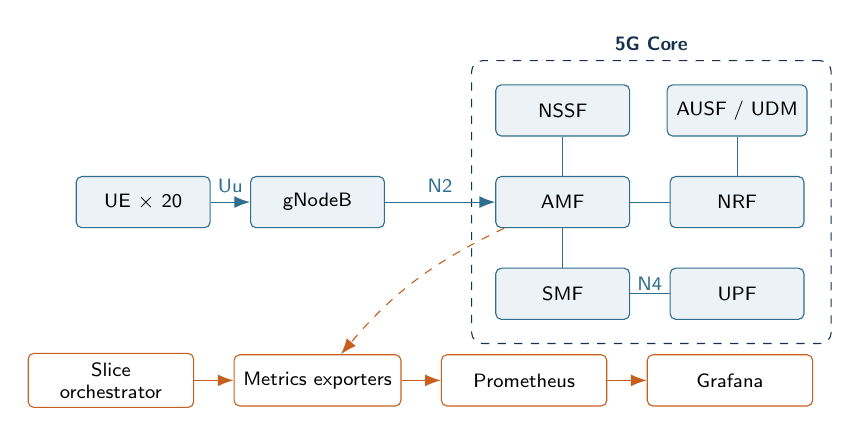
\begin{tikzpicture}[every node/.style={font=\scriptsize},node distance=5mm]
      \tikzstyle{box}=[draw=brandMid,fill=brandLight,rounded corners=2pt,
                       minimum height=6.5mm,minimum width=17mm,align=center]
      \tikzstyle{obs}=[draw=brandAccent,fill=white,rounded corners=2pt,
                       minimum height=6.5mm,minimum width=21mm,align=center]
      \node[box] (ue) {UE $\times$ 20};
      \node[box,right=of ue] (gnb) {gNodeB};
      \node[box,right=14mm of gnb] (amf) {AMF};
      \node[box,above=of amf] (nssf) {NSSF};
      \node[box,below=of amf] (smf) {SMF};
      \node[box,right=of amf] (nrf) {NRF};
      \node[box,above=of nrf] (ausf) {AUSF / UDM};
      \node[box,below=of nrf] (upf) {UPF};

      \draw[-{Latex[length=2mm]},brandMid] (ue)--(gnb) node[midway,above]{Uu};
      \draw[-{Latex[length=2mm]},brandMid] (gnb)--(amf) node[midway,above]{N2};
      \draw[-,brandMid] (amf)--(nssf);
      \draw[-,brandMid] (amf)--(smf);
      \draw[-,brandMid] (amf)--(nrf);
      \draw[-,brandMid] (nrf)--(ausf);
      \draw[-,brandMid] (smf)--(upf) node[midway,above,inner sep=1pt]{N4};

      \begin{scope}[on background layer]
        \node[draw=brandDark,dashed,rounded corners,fit=(nssf)(amf)(smf)(nrf)(ausf)(upf),
              inner sep=3mm,label={[font=\scriptsize\bfseries,brandDark]above:5G Core}] {};
      \end{scope}

      \node[obs,below=16mm of gnb] (exp) {Metrics exporters};
      \node[obs,right=of exp] (prom) {Prometheus};
      \node[obs,right=of prom] (graf) {Grafana};
      \node[obs,left=of exp] (orch) {Slice\\orchestrator};

      \draw[-{Latex[length=2mm]},brandAccent,dashed] (amf) to[bend right=12] (exp);
      \draw[-{Latex[length=2mm]},brandAccent] (exp)--(prom);
      \draw[-{Latex[length=2mm]},brandAccent] (prom)--(graf);
      \draw[-{Latex[length=2mm]},brandAccent] (orch)--(exp);
    \end{tikzpicture}
  \end{center}
  \vspace{-2mm}
  \begin{block}{Design principle}
    \small
    Telemetry flows in \textbf{one direction only}. The observability plane reads
    from the Core and never writes back into it, so monitoring cannot perturb the
    network under test.
  \end{block}
\end{frame}

%================================================================ 9 Functionalities
\begin{frame}{Functionalities of the Proposed System}
  \begin{columns}[T,onlytextwidth]
    \begin{column}{0.49\textwidth}
      \begin{block}{Deployment and validation}
        \small
        \begin{itemize}
          \item Reproducible, version-pinned environment
          \item Automated environment conformance checks
          \item Integrity gate in continuous integration
          \item Automated subscriber provisioning
        \end{itemize}
      \end{block}
      \begin{block}{Radio access and mobility}
        \small
        \begin{itemize}
          \item gNodeB--AMF signalling over SCTP/NGAP
          \item UE registration with 5G-AKA authentication
          \item Multiple UEs operating in parallel
        \end{itemize}
      \end{block}
    \end{column}
    \begin{column}{0.49\textwidth}
      \begin{block}{Observability}
        \small
        \begin{itemize}
          \item Metrics collected from every network function
          \item Dashboards for runtime network state
          \item Alert rules for availability and errors
          \item Timestamped evidence capture
        \end{itemize}
      \end{block}
      \begin{block}{Slice management}
        \small
        \begin{itemize}
          \item Two service types with distinct QoS
          \item Slice-labelled metrics
          \item Demand-based allocation with admission control
        \end{itemize}
      \end{block}
    \end{column}
  \end{columns}
\end{frame}

%================================================================ 10 Software/Tools
\begin{frame}{Software / Tools Requirements}
  \small
  \begin{columns}[T,onlytextwidth]
    \begin{column}{0.49\textwidth}
      \begin{block}{5G network stack}
        \renewcommand{\arraystretch}{1.15}
        \begin{tabular}{@{}ll@{}}
          free5GC & 5G Standalone Core\\
          UERANSIM & gNodeB and UE simulation\\
          gtp5g & User-plane kernel module\\
          MongoDB & Subscriber database\\
        \end{tabular}
      \end{block}
      \begin{block}{Platform}
        \renewcommand{\arraystretch}{1.15}
        \begin{tabular}{@{}ll@{}}
          Ubuntu 24.04 LTS & Host operating system\\
          Docker + Compose & Containerization\\
          Kubernetes & Orchestration (Phase 2)\\
        \end{tabular}
      \end{block}
    \end{column}
    \begin{column}{0.49\textwidth}
      \begin{block}{Observability and automation}
        \renewcommand{\arraystretch}{1.15}
        \setlength{\tabcolsep}{3pt}
        \begin{tabular}{@{}ll@{}}
          Prometheus & Metrics collection\\
          Grafana & Dashboards\\
          Python & Exporters, orchestrator\\
          Bash & Deployment automation\\
          Git / GitHub Actions & Version control, CI\\
        \end{tabular}
      \end{block}
      \begin{block}{Hardware baseline}
        \small
        x86\_64, $\geq$ 8 logical cores, $\geq$ 16 GB RAM,
        $\geq$ 100 GB SSD; bare-metal Linux required for the user plane.
      \end{block}
    \end{column}
  \end{columns}
\end{frame}

%================================================================ 11 Phase 2 progress: observability
\begin{frame}{Phase 2 Progress --- Observability Plane}
  \begin{columns}[T,onlytextwidth]
    \begin{column}{0.54\textwidth}
      \begin{block}{What was built}
        \small
        \begin{itemize}
          \item Native metrics enabled on every network function
          \item Continuous collection every 15 seconds
          \item Dashboards for registration, signalling and errors
          \item Alert rules for availability and failure rates
        \end{itemize}
      \end{block}
      \begin{block}{Why it matters}
        \small
        Deployment success is no longer inferred from container status ---
        it is measured from the network's own behaviour.
      \end{block}
    \end{column}
    \begin{column}{0.42\textwidth}
      \begin{block}{Signals collected}
        \small
        \begin{itemize}
          \item Registration and session procedures
          \item NAS and NGAP message rates
          \item Inter-function API latency
          \item Error responses by cause
        \end{itemize}
      \end{block}
    \end{column}
  \end{columns}
\end{frame}

%================================================================ 12 Key finding
\begin{frame}{Phase 2 Progress --- Key Finding}
  \begin{block}{Observation}
    \small
    Every metric exposed by the 5G Core was examined. \textbf{None of them
    identifies the network slice it belongs to.}
  \end{block}
  \begin{columns}[T,onlytextwidth]
    \begin{column}{0.46\textwidth}
      \begin{block}{Consequence}
        \small
        Per-slice assurance is impossible from native telemetry alone. One can
        see that the network is busy, but not \emph{which slice} is busy.
      \end{block}
    \end{column}
    \begin{column}{0.5\textwidth}
      \begin{block}{Resolution --- without modifying upstream code}
        \small
        Slice identity is recovered from the Core's own signalling records and
        joined with the subscriber database to produce genuinely
        \textbf{slice-labelled} metrics.
      \end{block}
    \end{column}
  \end{columns}
  \vfill
  \begin{center}
    \small\itshape
    This confirms an open problem identified in the literature survey: slicing is
    treated as configuration rather than as an observable, measurable resource.
  \end{center}
\end{frame}

%================================================================ 13 Slice allocation
\begin{frame}{Phase 2 Progress --- Slice-Aware Resource Allocation}
  \begin{center}
    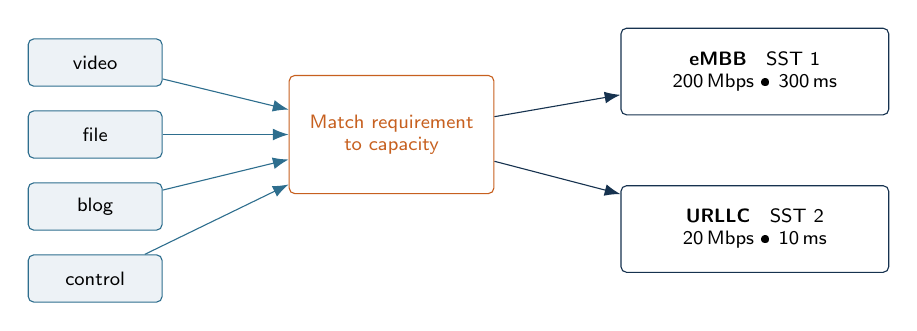
\begin{tikzpicture}[every node/.style={font=\scriptsize},node distance=7mm]
      \tikzstyle{t}=[draw=brandMid,fill=brandLight,rounded corners=2pt,
                     minimum height=6mm,minimum width=17mm,align=center]
      \tikzstyle{s}=[draw=brandDark,fill=white,rounded corners=2pt,
                     minimum height=11mm,minimum width=34mm,align=center]
      \node[t] (v) {video};
      \node[t,below=3mm of v] (f) {file};
      \node[t,below=3mm of f] (b) {blog};
      \node[t,below=3mm of b] (c) {control};
      \node[draw=brandAccent,fill=white,rounded corners=2pt,right=16mm of f,
            minimum height=15mm,minimum width=26mm,align=center,text=brandAccent]
            (dec) {Match requirement\\to capacity};
      \node[s,right=16mm of dec,yshift=8mm] (embb)
            {\textbf{eMBB} \; SST 1\\200\,Mbps \textbullet\ 300\,ms};
      \node[s,right=16mm of dec,yshift=-12mm] (urllc)
            {\textbf{URLLC} \; SST 2\\20\,Mbps \textbullet\ 10\,ms};
      \draw[-{Latex[length=2mm]},brandMid] (v)--(dec);
      \draw[-{Latex[length=2mm]},brandMid] (f)--(dec);
      \draw[-{Latex[length=2mm]},brandMid] (b)--(dec);
      \draw[-{Latex[length=2mm]},brandMid] (c)--(dec);
      \draw[-{Latex[length=2mm]},brandDark] (dec)--(embb);
      \draw[-{Latex[length=2mm]},brandDark] (dec)--(urllc);
    \end{tikzpicture}
  \end{center}
  \vspace{-1mm}
  \begin{columns}[T,onlytextwidth]
    \begin{column}{0.5\textwidth}
      \begin{block}{Allocation policy}
        \small
        Traffic is placed on the \emph{least specialised} slice that still meets
        its latency requirement, preserving scarce low-latency capacity.
      \end{block}
    \end{column}
    \begin{column}{0.46\textwidth}
      \begin{block}{Admission control}
        \small
        A demand is \textbf{refused} when no permitted slice has capacity
        remaining --- resources are finite and enforced.
      \end{block}
    \end{column}
  \end{columns}
\end{frame}

%================================================================ 14 Results
\begin{frame}{Results}
  \begin{columns}[T,onlytextwidth]
    \begin{column}{0.44\textwidth}
      \begin{block}{Deployment}
        \small
        \begin{itemize}
          \item 8 of 8 network functions registered
          \item 20 of 20 UEs registered successfully
          \item Two slices with distinct service types
          \item Environment reproduces identically
        \end{itemize}
      \end{block}
    \end{column}
    \begin{column}{0.52\textwidth}
      \begin{block}{Slice differentiation achieved}
        \scriptsize
        \renewcommand{\arraystretch}{1.2}
        \begin{tabular}{@{}lcc@{}}
          \toprule
          \textbf{Parameter} & \textbf{eMBB} & \textbf{URLLC}\\
          \midrule
          Service type (SST) & 1 & 2\\
          QoS identifier (5QI) & 9 & 82\\
          Priority (ARP) & 8 & 2\\
          Bandwidth ceiling & 200\,Mbps & 20\,Mbps\\
          Latency budget & 300\,ms & 10\,ms\\
          \bottomrule
        \end{tabular}
      \end{block}
    \end{column}
  \end{columns}
  \vfill
  \begin{block}{Verification}
    \small
    All figures are produced by automated checks and stored as timestamped
    evidence, so every result is reproducible rather than merely reported.
  \end{block}
\end{frame}

%================================================================ 15 Challenges
\begin{frame}{Challenges and Key Learnings}
  \small
  \renewcommand{\arraystretch}{1.3}
  \begin{tabular}{@{}p{0.42\textwidth}p{0.52\textwidth}@{}}
    \toprule
    \textbf{Challenge} & \textbf{Learning / Resolution}\\
    \midrule
    Metrics carry no slice identity
      & Recovered from signalling records instead of patching upstream code\\
    Authentication failures resembling wrong credentials
      & Root cause was a sequence-number mismatch --- symptoms can point away from the real fault\\
    Slice selection failing silently
      & Configuration must be consistent across \emph{every} network function\\
    Built-in counters drifting from reality
      & Independent ground truth is essential before trusting a dashboard\\
    User-plane module tied to the host kernel
      & Environment constraints must be validated before integration, not during\\
    \bottomrule
  \end{tabular}
\end{frame}

%================================================================ 16 Timeline
\begin{frame}{Timeline}
  \begin{center}
    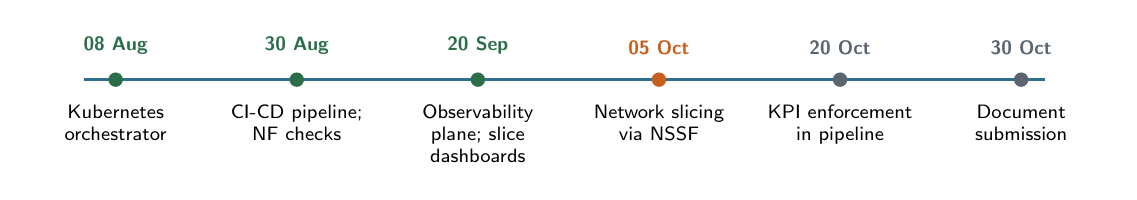
\begin{tikzpicture}[every node/.style={font=\scriptsize}]
      \draw[brandMid,line width=1pt] (0,0)--(12.2,0);
      \foreach \x/\d/\t/\col in {%
        0.4/08 Aug/Kubernetes orchestrator/okGreen,
        2.7/30 Aug/CI-CD pipeline; NF checks/okGreen,
        5.0/20 Sep/Observability plane; slice dashboards/okGreen,
        7.3/05 Oct/Network slicing via NSSF/brandAccent,
        9.6/20 Oct/KPI enforcement in pipeline/softGrey,
        11.9/30 Oct/Document submission/softGrey}{%
        \fill[\col] (\x,0) circle (2.6pt);
        \node[above=2mm of {(\x,0)},text=\col,font=\scriptsize\bfseries] {\d};
        \node[below=2mm of {(\x,0)},align=center,text width=20mm] {\t};
      }
    \end{tikzpicture}
  \end{center}
  \vfill
  \begin{center}
    \footnotesize
    {\color{okGreen}$\bullet$}~Completed \quad
    {\color{brandAccent}$\bullet$}~Current \quad
    {\color{softGrey}$\bullet$}~Planned
  \end{center}
\end{frame}

%================================================================ 17 Conclusion
\begin{frame}{Conclusion}
  \begin{columns}[T,onlytextwidth]
    \begin{column}{0.5\textwidth}
      \begin{block}{Achieved in this phase}
        \small
        \begin{itemize}
          \item Reproducible 5G Core and RAN deployment
          \item Continuous observability plane
          \item Slice-labelled metrics despite no native support
          \item Demand-based slice allocation with admission control
        \end{itemize}
      \end{block}
    \end{column}
    \begin{column}{0.48\textwidth}
      \begin{block}{Remaining work}
        \small
        \begin{itemize}
          \item KPI thresholds as pipeline pass/fail gates
          \item Automatic rollback on KPI regression
          \item Migration to Kubernetes orchestration
          \item Allocation driven by measured load
        \end{itemize}
      \end{block}
    \end{column}
  \end{columns}
  \vfill
  \begin{block}{Contribution}
    \small
    The framework moves 5G deployment from \emph{“the containers started”} to
    \emph{“the network is measurably serving each slice”} --- and the remaining
    work converts that observation into automated action.
  \end{block}
\end{frame}

%================================================================ 18 References
\begin{frame}{References}
  \tiny
  \begin{enumerate}\setlength{\itemsep}{1.4pt}
    \item Makani, S. T., \& Jangampeta, S. (2022). The Evolution of CI/CD Tools in DevOps from Jenkins to GitHub Actions. \emph{Int. J. of Computer Engineering}.
    \item Moravcik, M., Kontsek, M., Segec, P., \& Cymbalak, D. (2022). Kubernetes --- Evolution of Virtualization. \emph{ICETA}.
    \item Bhatia, A. (2025). Evolution of CI/CD in Cloud-Native Development. \emph{IJCTT}, 73(5), 155--161.
    \item Baqar, M., Naqvi, S., \& Khanda, R. (2025). AI-Augmented CI/CD Pipelines: From Code Commit to Production with Autonomous Decisions. \emph{PriMera Scientific Engineering}.
    \item Owobu, W. O., Gbenle, P., \& Alozie, C. E. (2025). The Evolution and Impact of Kubernetes in Modern Software Engineering.
    \item Rigneault, H., et al. (2023). Cloud Native Network Slice Orchestration in 5G and Beyond.
    \item Panek, M., Pomyka\l{}a, A., Jab\l{}o\'nski, I., \& Wo\'zniak, M. (2023). 5G/5G+ Network Management Employing AI-Based Continuous Deployment. \emph{Applied Soft Computing}.
    \item Motamary, S. (2023). A Deep Dive into CI/CD Pipelines Tailored for Telecom: Orchestrating Cloud-Native 5G Services with DevOps and Infrastructure Automation.
    \item Singirikonda, P. (2024). 5G-Enabled DevOps: Revolutionizing Integrated Communication and Networking Technologies for Faster Software Delivery.
    \item Davuluri, S. K., Challagulla, V., Mudapaka, V., \& Konka, U. (2025). AI-Driven DevOps in Telecommunications.
    \item Herrera, J. L., Montebugnoli, S., Scotece, D., Foschini, L., \& Bellavista, P. (2026). A Tutorial on O-RAN Deployment Solutions for 5G: From Simulation to Emulated and Real Testbeds. \emph{IEEE COMST}.
    \item Sufyan, A., Khan, K. B., Khashan, O. A., Mir, T., \& Mir, U. (2023). From 5G to Beyond 5G: A Comprehensive Survey of Wireless Network Evolution, Challenges, and Promising Technologies.
    \item Narasimhulu, M., Mounika, D. V., Varshini, P., Amarendra, K., \& Rao, T. K. R. K. (2023). Investigating the Impact of Containerization on the Deployment Process in DevOps.
    \item Sakinala, K. (2025). The Synergistic Impact of Artificial Intelligence on DevOps: A Comprehensive Review.
    \item Garcia, F. J., et al. (2025). 5G-CT: Automated Deployment and Over-the-Air Testing of End-to-End Open Radio Access Networks. \emph{IEEE}.
  \end{enumerate}
\end{frame}

%================================================================ 19 Thank You
\begin{frame}[plain]
  \vfill
  \begin{center}
    
\includegraphics[height=12mm]{assets/logo2.jpeg}\\[5mm]
    {\Huge\bfseries\color{brandDark} THANK YOU}\\[4mm]
    {\large Questions and Suggestions}\\[9mm]
    \small Team 23UG005 \quad\textbullet\quad Panel 4\\
    \small Project Guide: Ms.\ Pooja Gowda
  \end{center}
  \vfill
\end{frame}

\end{document}
